\chapter{Open Source Software for Causal Inference}\label{five}

\section{Towards ``Really Reproducible'' Research}

Electronic computation has had a transformative impact on the discipline of
statistics, both in the development of novel statistical methodology and the
practice of statistical data analysis. Modern statistical techniques rely
heavily upon the widespread availability of personal computers and
high-performance computing systems, and, today, some of the most well-known and
influential procedures for statistical estimation and inference --- including
ensemble machine learning~\citep{wolpert1992stacked, breiman1996stacked,
vdl2007super}, the jackknife~\citep{efron1981nonparametric}, and the
bootstrap~\citep{efron1981nonparametric, efron1994introduction,
davison1997bootstrap} --- presume the availability of significant computational
resources. The ease of access to and reliability of modern computing systems,
coupled with their ever-increasing capabilities, has allowed tremendous strides
in not only how statistical methods are developed but in the range of scientific
problems to which they may be applied. Despite these advances, critical lessons
and pratices for facilitating the reproducibility of findings from the
computational sciences, readily absorbed by allied disciplines, were left
largely unheeded by statisticians for most of the twentieth and early
twenty-first centuries.

An early call to embrace computing and programming was issued
by~\citet{tukey1962future}, who saw such activities as critical to the next
generation of developments in statistical data analysis. While Tukey's
prominence afforded his timely concerns visibility, only a very small fraction
of the total academic effort in statistics research became concentrated upon the
inception and improvement of standards for statistical programming, computing,
and graphics~\citep{becker1984s, becker1988new, ihaka1996r} or on the
complementary paradigms of literate programming~\citep{knuth1984literate} and
literate computing~\citep{perez2013literate}. Cross-talk between statistics and
related computationally intensive sciences led to further concern about the
state of reproducibility in computational research. For example, as lessons
learned from their development of \textit{Wavelab}, a robust software toolkit
for wavelet analysis, \citet{buckheit1995wavelab} bemoaned the lack of
availability of scientific software, remarking that the ``release of software
underlying scientific publication is the exception rather than the rule'' while
simultaneously observing that, with respect to scientific publications, ``the
actual scholarship is the complete software development environment and the
complete set of instructions which generated the figures.'' Fortunately, the
decades leading to the recent emergence of the interdisciplinary field of data
science~\citep{donoho2017fifty} have been marked by a renewed and fervent
interest in open source software development and reproducible research.

As we move into an era in which sophisticated statistical techniques are
routinely deployed for rigorously evaluating scientific claims of global
concern, such as the vaccine efficacy trials discussed in Chapters~\ref{two}
and~\ref{three}, the availability and adoption of robust statistical software
will undoubtedly play a central role in enhancing the transparency inherent to
the scientific process. That is, the conscientious use of modern statistical
methodology alone has become insufficient for the practice of open science. For
transparent scientific practice to thrive, user-friendly software will need to
become the norm, rather than the exception, as has historically been the
case~\citep{stromberg2004write, pullenayegum2016knowledge}. Such software is
characterized by at least five essential characteristics.
\begin{enumerate}[topsep=0.5pt,itemsep=0pt,partopsep=1ex,parsep=1ex]
  \item Clear, easily accessible, highly detailed documentation of all
       code-derived interfaces and objects, whether developer-oriented or
       user-facing.
   \item Rigorous and focused testing to assess programmatic procedures (e.g.,
       functions, classes, methods) and data structures (e.g., the
       ubiquitous data frame).
  \item In-depth examples using literate programming documents that blend
      executable code with prose (e.g., \texttt{RMarkdown}~\citep{xie2018r}) or
      literate computing notebooks that promote the interactive development of
      computation \textit{informed by data} (e.g., Jupyter
      notebooks~\citep{kluyver2016jupyter, granger2021jupyter}).
  \item Open source development, embodying an ongoing, continuous, public
       peer review of the research product.
  \item The automated, near-constant monitoring of software quality through
      continuous integration services, ensuring accessibility across diverse
      computer systems and architectures.
\end{enumerate}
By displaying these characteristics, software for statistics can empower the
scientific community --- and possibly even the public at large --- to directly
access the published results of scientific investigations. Practices for
reproducible research in statistics and allied computational sciences have been
the subject of much discussion~\citep[e.g.,][]{peng2009reproducible,
peng2011reproducible, stodden2014implementing, kitzes2017practice,
millman2018developing}; however, in many academic circles, the core aspects of
software development are still viewed as an ancillary activity, rather than as
a primary pursuit.

As the fields of statistics and data science continue to co-develop in the
coming decades, statisticians will be challenged by questions that highlight the
importance of software to the field. Such questions include, for example, (1)
how a theorem, or similar mathematical result, can significantly impact science
\textit{except through software}, or (2) in what ways software implementations
can readily reveal important insights about the computational bottlenecks of
newly developed statistical methodology. Recalling an anecdote
of~\citet{buckheit1995wavelab}, we note that, without continued investment in
the development and promotion of open source software standards, ``a year [will
continue to be] a long time in this business,'' as the application of existing
statistical methodology to newly procured datasets will be marked by the
unreliability and instability of accompanying software. We hope that such
occurrences will become exceedingly rare. To that end, we next present three
open source software packages, each developed to implement distinct statistical
methods described in this greater body of work. Written for the \texttt{R}
programming language~\citep{R}, the unrestricted source code for each package is
available on the collaborative programming platform GitHub; moreover, each
package is accompanied by online documentation, a suite of unit tests, and
automated quality control through continuous integration services.

\section{The \texttt{txshift} \texttt{R} Package}\label{pkg_txshift}

\subsection{Summary}

Statistical causal inference has traditionally focused on effects defined by
inflexible static interventions, applicable only to binary or categorical
exposures. The evaluation of such interventions is often plagued by many
problems, both theoretical (e.g., non-identification) and practical (e.g.,
positivity violations); however, stochastic interventions provide a promising
solution to these fundamental issues~\citep{diaz2018stochastic}. The
\texttt{txshift} \texttt{R} package provides researchers in (bio)statistics,
epidemiology, health policy, economics, and related disciplines with access to
state-of-the-art statistical methodology for evaluating the causal effects of
stochastic shift interventions on \textit{continuous-valued} exposures.
\texttt{txshift} estimates the causal effects of modified treatment policies (or
``feasible interventions''), which take into account the natural value of an
exposure in assigning an intervention level. To accommodate use in study designs
incorporating outcome-dependent two-phase sampling (e.g., case-control), the
package provides two types of modern corrections, both rooted in semiparametric
theory, for constructing unbiased and efficient estimates, despite the
significant limitations induced by such designs. Thus, \texttt{txshift} makes
possible the estimation of the causal effects of stochastic interventions in
experimental and observational study settings subject to real-world design
limitations that commonly arise in modern scientific practice.

\subsection{Statement of Need}

Researchers seeking to build upon or apply cutting-edge statistical approaches
for causal inference often face significant obstacles: such methods are usually
not accompanied by robust, well-tested, and well-documented software packages.
Yet coding such methods from scratch is often impractical for the applied
researcher, as understanding the theoretical underpinnings of these methods
requires advanced training, severely complicating the assessment and testing of
bespoke causal inference software. What's more, even when such software tools
exist, they are usually minimal implementations, providing support only for
deploying the statistical method in problem settings untouched by the
complexities of real-world data. The \texttt{txshift} \texttt{R} package solves
this problem by providing an open source tool for evaluating the causal effects
of flexible, stochastic interventions, applicable to categorical or
continuous-valued exposures, while providing corrections for appropriately
handling data generated by commonly used but complex two-phase sampling designs.

\subsection{Background}

Causal inference has traditionally focused on the effects of static
interventions, under which the magnitude of the exposure is set to a fixed,
prespecified value for each unit. The evaluation of such interventions faces
a host of issues, among them non-identification, violations of the assumption of
positivity, and inefficiency. Stochastic interventions provide a promising
solution to these fundamental issues by allowing for the target parameter to be
defined as the mean counterfactual outcome under a hypothetically shifted
version of the observed exposure distribution~\citep{diaz2012population}.
Modified treatment policies, a particular class of such interventions, may be
interpreted as shifting the natural exposure level at the level of a given
observational unit~\citep{haneuse2013estimation, diaz2018stochastic}.

Despite the promise of such advances in causal inference, real data analyses are
often further complicated by economic constraints, such as when the primary
variable of interest is far more expensive to collect than auxiliary covariates.
Two-phase sampling is often used to bypass these limitations --- unfortunately,
these sampling schemes produce side effects that require further adjustment when
formal statistical inference is the principal goal of a study. Among the rich
literature on two-phase designs, \citet{rose2011targeted2sd} stand out for
providing a study of nonparametric efficiency theory under a broad class of
two-phase designs. Their work provides guidance on constructing efficient
estimators of causal effects under general two-phase sampling designs.

\subsection{\texttt{txshift}'s Scope}

Building on these prior works, \citet{hejazi2020efficient} outlined a novel
approach for use in such settings: augmented targeted minimum loss (TML) and
one-step estimators for the causal effects of stochastic interventions, with
guarantees of consistency, efficiency, and multiple robustness despite the
presence of two-phase sampling. These authors further outlined a technique that
summarizes the effect of shifting an exposure variable on the outcome of
interest via a nonparametric working marginal structural model, analogous to
a dose-response analysis. The \texttt{txshift} software package, for the
\texttt{R} language and environment for statistical computing~\citep{R},
implements this methodology.

\texttt{txshift} is designed to facilitate the construction of TML and one-step
estimators of the causal effects of modified treatment policies that shift the
observed exposure value up (or down) by an arbitrary scalar $\delta$, which may
possibly take into account the natural value of the exposure (and, in future
versions, the covariates). The \texttt{R} package includes tools for deploying
these efficient estimators under outcome-dependent two-phase sampling designs,
with two types of corrections: (1) a reweighting procedure that introduces
inverse probability of censoring weights directly into relevant loss functions,
as discussed in \citet{rose2011targeted2sd}; as well as (2) an augmented
efficient influence function estimating equation, studied more thoroughly by
\citet{hejazi2020efficient}. \texttt{txshift} integrates with the \texttt{sl3}
package~\citep{coyle2021sl3} to allow for ensemble machine learning to be
leveraged in the estimation of nuisance parameters. What's more, the
\texttt{txshift} package draws on both the
\texttt{hal9001}~\citep{coyle2021hal9001,hejazi2020hal9001} and
\texttt{haldensify}~\citep{hejazi2021haldensify} \texttt{R} packages to allow
each of the efficient estimators to be constructed in a manner consistent with
the methodological and theoretical advances of~\citet{hejazi2020efficient},
which require fast convergence rates of nuisance parameters to their true
counterparts for efficiency of the resultant estimator.

\subsection{Availability}

The \texttt{txshift} package has been made publicly available both via
GitHub (\url{https://github.com/nhejazi/txshift}) and the Comprehensive
\texttt{R} Archive Network (\url{https://CRAN.R-project.org/package=txshift}).
Use of the \texttt{txshift} package has been extensively documented in the
package's \texttt{README}, two vignettes, and its \texttt{pkgdown} documentation
website (\url{https://code.nimahejazi.org/txshift}).

\section{The \texttt{medshift} \texttt{R} Package}\label{pkg_medshift}

\subsection{Background}

This \texttt{R} package aims to provide tools for assessing the population
intervention direct effect and the population intervention indirect effect,
based on the effect decomposition of the population intervention effect
introduced in~\citet{diaz2020causal}.

To proceed, we will use as our running example a simple data set from an
observational study of the relationship between BMI and kids behavior,
distributed as part of the \texttt{mma} \texttt{R} package on the Comprehensive
\texttt{R} Archive Netowrk (\url{https://CRAN.R-project.org/package=mma}).
First, a bit of quick programmatic housekeepking for this data example.

\begin{lstlisting}
# preliminaries
library(data.table)
library(dplyr)
library(tidyr)
library(sl3)
library(medshift)
library(mma)
\end{lstlisting}

The documentation for the data set describes it as a ``database obtained from
the Louisiana State University Health Sciences Center, New Orleans, by  Dr.
Richard Scribner. He  explored the relationship  between BMI and kids behavior
through a survey at children, teachers and parents in Grenada in 2014. This data
set includes $691$ observations and $15$ variables.''

Unfortunately, the data set contains a few observations with missing values. As
these are unrelated to the object of our analysis, we'll simply remove these for
the time being. Note that in a real data analysis, we might consider strategies
to fully make of the observed data, perhaps by imputing missing values. For now,
we simply remove the incomplete observations, resulting in a data set with fewer
observations (now $567$ units) but otherwise the same structure as the original.

\begin{lstlisting}
# load and clean up data
data(weight_behavior)
weight_behavior_complete <- weight_behavior %>%
  drop_na() %>%
  mutate(as.numeric(sports) - 1)
dim(weight_behavior_complete)
head(weight_behavior_complete)

##        bmi  age sex  race numpeople car gotosch snack tvhours cmpthours
## 1 18.20665 12.2   F OTHER         5   3       2     1       4         0
## 2 22.78401 12.8   M OTHER         4   3       2     1       4         2
## 4 25.56754 12.1   M OTHER         2   3       2     1       0         2
## 5 15.07408 12.3   M OTHER         4   1       2     1       2         1
## 6 22.98338 11.8   M OTHER         4   1       1     1       4         3
## 8 19.15658 12.1   F OTHER         3   3       2     1       0         0
##   cellhours sports exercises sweat overweigh
## 1         0      1         2     1         0
## 2         0      0         8     2         0
## 4         0      1         9     1         1
## 5         3      0        12     1         0
## 6         2      0         1     1         0
## 8         1      0         1     3         0
\end{lstlisting}

For the analysis of this observational data set, we focus on the effect of
participating in a sports team (\texttt{sports}) on the BMI of children
(\texttt{bmi}), taking several related covariates as mediators (\texttt{snack},
\texttt{exercises}, \texttt{overweigh}) and all other collected covariates as
potential confounders. Considering an NPSEM, we separate the observed variables
from the data set into their corresponding nodes as follows.

\begin{lstlisting}
Y <- weight_behavior_complete$bmi
A <- weight_behavior_complete$sports
Z <- weight_behavior_complete %>%
  select(snack, exercises, overweigh)
W <- weight_behavior_complete %>%
  select(age, sex, race, numpeople, car, gotosch, tvhours, cmpthours,
         cellhours, sweat)
\end{lstlisting}

Finally, in our analysis, we consider an incremental propensity score
intervention (IPSI), as first proposed by~\citet{kennedy2017nonparametric},
wherein the \textit{odds of participating in a sports team} is modulated by
a fixed amount ($0 \leq \delta \leq \infty$), specified \textit{a priori}, for
each individual. Such an intervention may be interpreted as the effect of
a school program that motivates children to participate in sports teams. To
exemplify our approach, we postulate a motivational intervention that
\textit{triples the odds} of participating in a sports team for each individual:
\begin{lstlisting}
delta_shift_ipsi <- 3
\end{lstlisting}

To easily incorporate ensemble machine learning into the estimation procedure,
we rely on the facilities provided in the \texttt{sl3} \texttt{R}
package (\url{https://tlverse.org/sl3})~\citep{coyle2021sl3}.
We construct an ensemble learner using a handful of popular machine learning
algorithms below.

\begin{lstlisting}
# SL learners used for continuous data (nuisance parameter M)
xgb_contin_lrnr <- Lrnr_xgboost$new(
  nrounds = 50, objective = "reg:linear"
)
enet_contin_lrnr <- Lrnr_glmnet$new(
  alpha = 0.5, family = "gaussian", nfolds = 3
)
lasso_contin_lrnr <- Lrnr_glmnet$new(
  alpha = 1, family = "gaussian", nfolds = 3
)
fglm_contin_lrnr <- Lrnr_glm_fast$new(family = gaussian())
contin_lrnr_lib <- Stack$new(
  enet_contin_lrnr, lasso_contin_lrnr,
  fglm_contin_lrnr, xgb_contin_lrnr
)
sl_contin_lrnr <- Lrnr_sl$new(
  learners = contin_lrnr_lib,
  metalearner = Lrnr_nnls$new()
)
# SL learners used for binary data (nuisance parameters G and E)
xgb_binary_lrnr <- Lrnr_xgboost$new(
  nrounds = 50, objective = "reg:logistic"
)
enet_binary_lrnr <- Lrnr_glmnet$new(
  alpha = 0.5, family = "binomial", nfolds = 3
)
lasso_binary_lrnr <- Lrnr_glmnet$new(
  alpha = 1, family = "binomial", nfolds = 3
)
fglm_binary_lrnr <- Lrnr_glm_fast$new(family = binomial())
binary_lrnr_lib <- Stack$new(
  enet_binary_lrnr, lasso_binary_lrnr,
  fglm_binary_lrnr, xgb_binary_lrnr
)
logistic_metalearner <- make_learner(
  Lrnr_solnp, metalearner_logistic_binomial, loss_loglik_binomial
)
sl_binary_lrnr <- Lrnr_sl$new(
  learners = binary_lrnr_lib,
  metalearner = logistic_metalearner
)
\end{lstlisting}

\subsection{Population Intervention Effect Decomposition}

We may decompose the population intervention effect (PIE) in terms of a
\textit{population intervention direct effect} (PIDE) and a \textit{population
intervention indirect effect} (PIIE):
\begin{equation*}
  \overbrace{\mathbb{E}\{Y(A_\delta, Z(A_\delta)) -
    Y(A_\delta, Z)\}}^{\text{PIIE}} +
    \overbrace{\mathbb{E}\{Y(A_\delta, Z) - Y(A, Z)\}}^{\text{PIDE}}.
\end{equation*}

This decomposition of the PIE as the sum of the population intervention direct
and indirect effects has an interpretation analogous to the corresponding
standard decomposition of the average treatment effect. In the sequel, we will
compute each of the components of the direct and indirect effects above using
appropriate estimators as follows.

\begin{itemize}[topsep=0pt,itemsep=0pt,partopsep=1ex,parsep=1ex]
\item For $\mathbb{E}\{Y(A, Z)\}$, the sample mean $\frac{1}{n}\sum_{i=1}^n
  Y_i$ is sufficient;
\item for $\mathbb{E}\{Y(A_{\delta}, Z)\}$, an efficient one-step estimator for
  the effect of a joint intervention altering the exposure mechanism but not the
  mediation mechanism, as proposed in~\citet{diaz2020causal}; and,
\item for $\mathbb{E}\{Y(A_{\delta}, Z_{A_{\delta}})\}$, an efficient one-step
  estimator for the effect of a joint intervention on both the exposure and and
  mediator(s), as proposed in~\citet{kennedy2017nonparametric} and implemented
  in the \texttt{npcausal} \texttt{R} package
  (\url{https://github.com/ehkennedy/npcausal}).
\end{itemize}

\subsection{Estimating the Effect Decomposition Term}

As given in~\citet{diaz2020causal}, the statistical functional identifying the
decomposition term that appears in both the PIDE and PIIE
$\mathbb{E}\{Y(A_{\delta}, Z)\}$, which corresponds to altering the exposure
mechanism while keeping the mediation mechanism fixed, is
\begin{equation*}
  \theta_0(\delta) = \int m_0(a, z, w) g_{0,\delta}(a \mid w) p_0(z, w)
    d\nu(a, z, w),
\end{equation*}
for which a one-step estimator is available. The corresponding \textit{efficient
influence function} (EIF) with respect to the nonparametric model $\mathcal{M}$
is $D_{\eta,\delta}(o) = D^Y_{\eta,\delta}(o)
+ D^A_{\eta,\delta}(o) + D^{Z,W}_{\eta,\delta}(o) - \theta(\delta)$. The
one-step estimator may be computed using the EIF estimating equation, making use
of cross-fitting~\citep{zheng2011cross,chernozhukov2018double} to circumvent any
need for entropy conditions (i.e., Donsker class restrictions). The resultant
estimator is
\begin{equation*}
  \hat{\theta}(\delta) = \frac{1}{n} \sum_{i = 1}^n D_{\hat{\eta}_{j(i)},
  \delta}(O_i) = \frac{1}{n} \sum_{i = 1}^n \left\{ D^Y_{\hat{\eta}_{j(i)},
  \delta}(O_i) + D^A_{\hat{\eta}_{j(i)}, \delta}(O_i) +
  D^{Z,W}_{\hat{\eta}_{j(i)}, \delta}(O_i) \right\},
\end{equation*}
which is implemented in the \texttt{medshift} \texttt{R} package. We make use of
that implementation to estimate $\mathbb{E}\{Y(A_{\delta}, Z)\}$ via its
one-step estimator $\hat{\theta}(\delta)$, as demonstrated below.

\begin{lstlisting}
# let's compute the parameter where A (but not Z) are shifted
theta_eff <- medshift(
  W = W, A = A, Z = Z, Y = Y,
   delta = delta_shift_ipsi,
   g_learners = sl_binary_lrnr,
   e_learners = sl_binary_lrnr,
   m_learners = sl_contin_lrnr,
   phi_learners = Lrnr_hal9001$new(),
   estimator = "onestep",
   estimator_args = list(cv_folds = 3)
)
summary(theta_eff)
\end{lstlisting}

\subsection{Estimating the Direct Effect}

Recall that, based on the decomposition outlined previously, the population
intervention direct effect may be denoted $\beta_{\text{PIDE}}(\delta) =
\theta_0(\delta) - \mathbb{E}Y$. Thus, an estimator of the PIDE,
$\hat{\beta}_{\text{PIDE}}(\delta)$ may be expressed as a composition of
estimators of its constituent parameters:
\begin{equation*}
  \hat{\beta}_{\text{PIDE}}({\delta}) = \hat{\theta}(\delta) -
  \frac{1}{n} \sum_{i = 1}^n Y_i.
\end{equation*}

Based on the above, we may construct an estimator of the PIDE using quantities
already computed. The convenience function below applies the simple delta method
required in the case of a linear contrast between the two constituent
parameters:
\begin{lstlisting}
# convenience function to compute inference via delta method: EY1 - EY0
linear_contrast <- function(params, eifs, ci_level = 0.95) {
  # bounds for confidence interval
  ci_norm_bounds <- c(-1, 1) * abs(qnorm(p = (1 - ci_level) / 2))
  param_est <- params[[1]] - params[[2]]
  eif <- eifs[[1]] - eifs[[2]]
  se_eif <- sqrt(var(eif) / length(eif))
  param_ci <- param_est + ci_norm_bounds * se_eif
  # parameter and inference
  out <- c(param_ci[1], param_est, param_ci[2])
  names(out) <- c("lwr_ci", "param_est", "upr_ci")
  return(out)
}
\end{lstlisting}

With the above convenience function in hand, we'll construct or extract the
necessary components from existing objects and simply apply the function:
\begin{lstlisting}
# parameter estimates and EIFs for components of direct effect
EY <- mean(Y)
eif_EY <- Y - EY
params_de <- list(theta_eff$theta, EY)
eifs_de <- list(theta_eff$eif, eif_EY)

# direct effect = EY - estimated quantity
de_est <- linear_contrast(params_de, eifs_de)
de_est
##       lwr_ci    param_est       upr_ci
##       -0.4961   -0.0073         0.4815
\end{lstlisting}

As given above, we have for our estimate of the direct effect
$\hat{\beta}_{\text{PIDE}}({\delta}) = -0.007$.

\section{The \texttt{haldensify} \texttt{R} Package}\label{pkg_haldensify}

\subsection{Statement of Need}

In causal inference problems, both classical estimators (e.g., based on inverse
probability weighting) and doubly robust estimators (e.g., one-step estimation,
targeted minimum loss estimation) require estimation of the propensity score, a
nuisance parameter corresponding to the treatment mechanism. While exposures of
interest may often be continuous-valued, most approaches opt to discretize the
exposure so as to estimate effects based on categorical exposures --- such
a simplification is often done out of convenience, to avoid estimation of the
\textit{generalized propensity score}~\citep{hirano2004propensity,
imai2004causal}, which is a conditional density function. The
\texttt{haldensify} package introduces a flexible approach for estimating such
conditional density functions, using the highly adaptive lasso (HAL),
a nonparametric regression function that has been proven to converge to a given
target function(al) at $n^{-1/3}$-rate under minimal conditions.

Consider data generated by typical cohort sampling $O = (W, A, Y)$, where $W$ is
a vector of baseline covariates, A is a continuous-valued exposure, and $Y$ is
an outcome of interest. Estimation of the generalized propensity score $g_{0,A}$
corresponds to estimating the conditional density of $A$ given $W = w$. A simple
strategy for estimating this nuisance function is to assume a parametric working
model and use parametric regression to generate suitable density estimates. For
example, one could operate under the working assumption that $A$ given $W$
follows a normal distribution with homoscedastic variance and mean
$\sum_{j=1}^p \beta_j \phi_j(W)$, where $\phi = (\phi_j : j)$ are user-selected
basis functions and $\beta = (\beta_j : j)$ are unknown regression parameters.
In this case, a density estimate would be generated by fitting a linear
regression of $A$ on $\phi(W)$ to estimate the conditional mean of $A$ given
$W$, paired with an estimate of the variance of $A$. Then, the estimated
conditional density would be given by the density of a Gaussian distribution
evaluated at these estimates. Unfortunately, most such approaches do not allow
for flexible modeling of $g_{0,A}$. This motivated our development of a novel
and flexible procedure for constructing conditional density estimates
$g_{n,A}(a \mid w)$ of $A$ given $W = w$ (possibly subject to observation-level
weights), evaluated at $a \in \mathcal{A}$.

\subsection{Conditional Density Estimation by Pooled Hazard Regression}

As consistent estimation of the generalized propensity score is an integral part
of constructing estimators of the causal effects of continuous-valued exposures,
our conditional density estimator, built around the HAL regression function, may
be quite useful in flexibly constructing such estimates. We note that proposals
for the data adaptive estimation of such quantities are sparse in the
literature~\citep[e.g.,][]{zhu2015boosting}. Notably, \citet{diaz2011super} gave
a proposal for constructing semiparametric estimators of such a target quantity
based on exploiting the relationship between the hazard and density functions.
Our proposal builds upon theirs in several key ways.
\begin{enumerate}[topsep=0.5pt,itemsep=0pt,partopsep=1ex,parsep=1ex]
  \item We adjust their algorithm so as to incorporate sample-level weights,
     necessary for making use of sample-level weights (e.g., inverse probability
     of censoring weighting).
  \item We replace the use of arbitrary classification models with the highly
  adaptive lasso.
\end{enumerate}
While our first modification is general and may be applied to the estimation
strategy of~\citet{diaz2011super}, our latter contribution requires adjusting
the penalization aspect of HAL regression models so as to respect the use of
a loss function appropriate for density estimation on the hazard scale.

To build an estimator of a conditional density, \citet{diaz2011super} considered
discretizing the observed $a \in A$ based on a number of bins $T$ and a binning
procedure (e.g., including the same number of points in each bin or forcing
bins to be of the same length). We note that the choice of the tuning parameter
$T$ corresponds roughly to the choice of bandwidth in classical kernel density
estimation; this will be made clear upon further examination of the proposed
algorithm. The data $\{A, W\}$ are reformatted such that the hazard of an
observed value $a \in A$ falling in a given bin may be evaluated via standard
classification techniques. In fact, this proposal may be viewed as
a re-formulation of the classification problem into a corresponding set of
hazard regressions:
\begin{align*}
   \mathbb{P} (A \in [\alpha_{t-1}, \alpha_t) \mid W) = &\mathbb{P} (A \in
   [\alpha_{t-1}, \alpha_t) \mid A \geq \alpha_{t-1}, W)\\ &\times
   \prod_{j = 1}^{t -1} \{1 - \mathbb{P} (A \in [\alpha_{j-1}, \alpha_j)
   \mid A \geq \alpha_{j-1}, W) \},
\end{align*}
where the probability that a value of $A \in \mathcal{A}$ falls in a bin
$[\alpha_{t-1}, \alpha_t)$ may be directly estimated from a standard
classification model. The likelihood of this model may be re-expressed in terms
of the likelihood of a binary variable in a data set expressed through
a repeated measures structure. Specifically, this re-formatting procedure is
carried out by creating a data set in which any given observation $A_i$ appears
(repeatedly) for as many intervals $[\alpha_{t-1}, \alpha_t)$ that there are
prior to the interval to which the observed $a$ belongs. A new binary outcome
variable, indicating $A_i \in [\alpha_{t-1}, \alpha_t)$, is recorded as part of
this new data structure. With the re-formatted data, a pooled hazard regression,
spanning the support of $A$ is then executed. Finally, the conditional density
estimator
\begin{equation*}
   g_{n, \alpha}(A \mid W) = \frac{\mathbb{P}(A \in [\alpha_{t-1}, \alpha_t)
      \mid W)}{(\alpha_t - \alpha_{t-1})},
\end{equation*}
for $\alpha_{t-1} \leq a \le \alpha_t$, may be constructed. As part of this
procedure, the hazard estimates are mapped to density estimates through
rescaling of the estimates by the bin size ($\alpha_t - \alpha_{t-1}$).

In its original proposal, a key element of this procedure was the use of any
arbitrary classification procedure for estimating $\mathbb{P}(A \in
[\alpha_{t-1}, \alpha_t) \mid W)$, facilitating the incorporation of flexible,
data adaptive estimators. We alter this proposal in two ways.
\begin{enumerate}[topsep=0.5pt,itemsep=0pt,partopsep=1ex,parsep=1ex]
  \item Replace the arbitrary estimator of $\mathbb{P}(A \in [\alpha_{t-1},
      \alpha_t) \mid W)$ with HAL regression~\citep{vdl2015generally,
      benkeser2016highly,vdl2017generally}, as implemented in the
      \texttt{hal9001} \texttt{R} package~\citep{coyle2021hal9001,
      hejazi2020hal9001}.
  \item Accommodate the use of sample-level weights, making it possible for
     the resultant conditional density estimator to achieve a convergence rate
     with respect to a loss-based dissimilarity of
     $n^{-1/3}$~\citep{bibaut2019fast}.
\end{enumerate}

Our procedure alters the HAL regression function to use a loss function tailored
for estimation of the hazard, invoking $\ell_1$-penalization in a manner
consistent with this loss.

\subsection{Code Demonstration}

First, let's load a few required packages, set a seed to make our example
reproducible, and generate some very simple, simulated example data.

\begin{lstlisting}
library(haldensify)
library(data.table)
library(ggplot2)
set.seed(75681)

make_example_data <- function(n_obs) {
  W <- runif(n_obs, -4, 4)
  A <- rnorm(n_obs, mean = W, sd = 0.25)
  dat <- as.data.table(list(A = A, W = W))
  return(dat)
}

# number of observations in our simulated dataset
n_obs <- 200
example_data <- make_example_data(n_obs)

# let's take a quick look at the data
head(example_data)

##             A           W
## 1:  2.3063922  2.24687273
## 2:  0.9297479  0.91025531
## 3: -3.2443382 -2.98696024
## 4: -0.1842217 -0.01204378
## 5:  3.2756387  3.59166824
## 6: -2.9132139 -3.02363838
\end{lstlisting}

The function \texttt{make\_example\_data()}, defined below, generates a baseline
covariate $W$ and a continuous-valued exposure variable $A$, whose mean is a
function of $W$.

Next, we'll fit our pooled hazards conditional density estimator via the
\texttt{haldensify()} function. Based on underlying theory and simulation
experiments, we recommend setting a relatively large number of bins and using a
binning strategy compatible with the large number of bins.

\begin{lstlisting}
haldensify_fit <- haldensify(
  A = example_data[["A"]],
  W = example_data[["W"]],
  n_bins = c(10, 20),
  grid_type = "equal_range",
  lambda_seq = exp(seq(-0.1, -10, length = 500)),
  # the following are passed to hal9001::fit_hal() internally
  max_degree = 5,
  num_knots = NULL,
  smoothness_orders = 0,
  reduce_basis = 1 / sqrt(n_obs)
)

# print the output object
haldensify_fit

## HAL Conditional Density Estimation
## Number of bins over support of A: 20
## CV-selected lambda: 4e-04
## Summary of fitted HAL:
##         coef                term
##  1:  4.015834         (Intercept)
##  2:  8.219963  [ I(W >= -3.305) ]
##  3:  7.080282  [ I(bin_id >= 9) ]
##  4: -6.906777  [ I(W >= -3.393) ]
##  5:  6.111346  [ I(bin_id >= 7) ]
##  6:  5.984919   [ I(W >= 0.474) ]
##  7:  5.615845  [ I(bin_id >= 2) ]
##  8:  5.536335  [ I(bin_id >= 4) ]
##  9:  5.375681 [ I(bin_id >= 13) ]
## 10:  5.270633  [ I(W >= -0.267) ]
\end{lstlisting}

Having constructed the conditional density estimator, we can examine the
empirical risk over the grid of choices of the $\ell_1$ regularization parameter
$\lambda$. To do this, we can simply call the available \texttt{plot()} method,
which uses the cross-validated conditional density fit stored in the
\texttt{haldensify} object. For example,

\begin{lstlisting}
plot(haldensify_fit)
\end{lstlisting}

The empirical risk curve of the conditional density estimates across differing
values of $\lambda$ are visualized in Figure~\ref{fig:haldensify_risk}.
\begin{figure}[H]
  \centering
  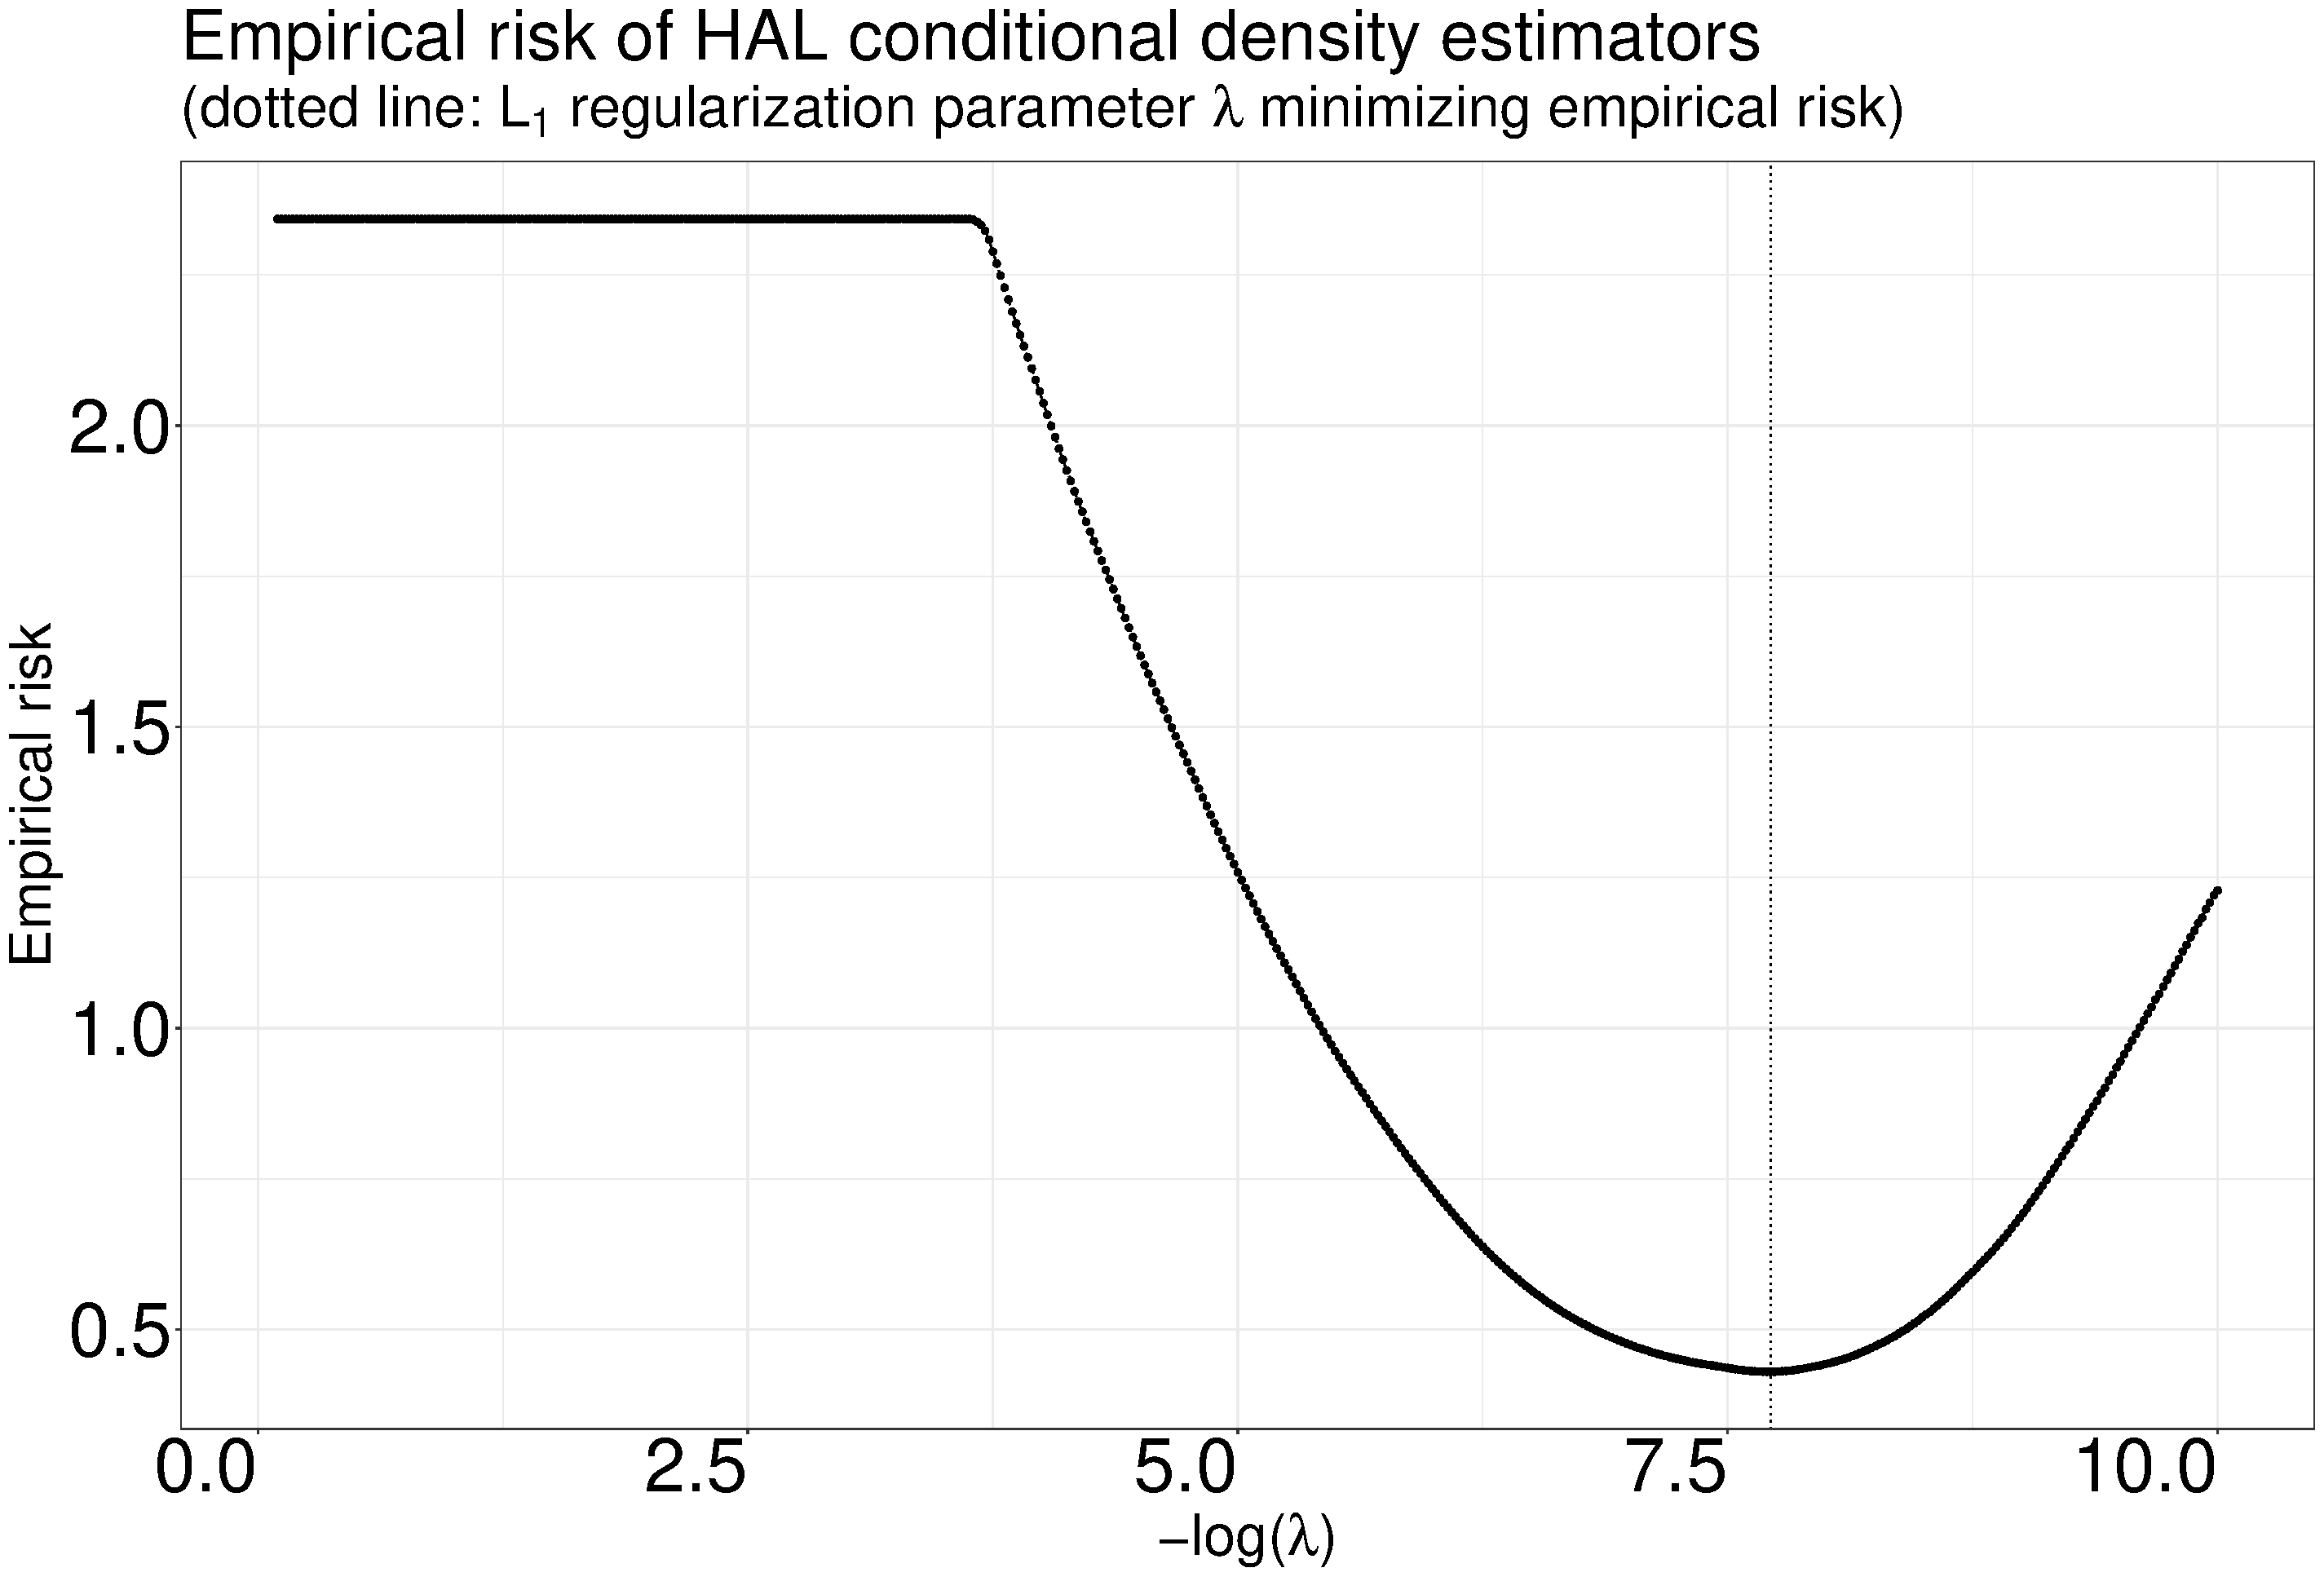
\includegraphics[scale=0.28]{haldensify_risk}
  \caption{Empirical risk of the estimated conditional density $g_{n,A}$ across
      a grid in the regularization parameter $\lambda$.}
  \label{fig:haldensify_risk}
\end{figure}

Finally, we can predict the conditional density over the grid of observed values
$A$ across different elements of the support $W$. We do this using the
\texttt{predict()} method of \texttt{haldensify} and plot the results below.

\begin{lstlisting}
# predictions to recover conditional density of A|W
new_a <- seq(-4, 4, by = 0.05)
new_dat <- as.data.table(list(
  a = new_a,
  w_neg = rep(-2, length(new_a)),
  w_zero = rep(0, length(new_a)),
  w_pos = rep(2, length(new_a))
))
new_dat[, pred_w_neg := predict(haldensify_fit,
                                new_A = new_dat[["a"]],
                                new_W = new_dat[["w_neg"]])]
new_dat[, pred_w_zero := predict(haldensify_fit,
                                 new_A = new_dat[["a"]],
                                 new_W = new_dat[["w_zero"]])]
new_dat[, pred_w_pos := predict(haldensify_fit,
                                new_A = new_dat[["a"]],
                                new_W = new_dat[["w_pos"]])]

# visualize results
dens_dat <-  melt(
  new_dat,
  id = c("a"),
  measure.vars = c("pred_w_pos", "pred_w_zero", "pred_w_neg")
)
p_dens <- ggplot(dens_dat, aes(x = a, y = value, colour = variable)) +
  geom_point() +
  geom_line() +
  stat_function(fun = dnorm, args = list(mean = -2, sd = 0.25),
             colour = "blue", linetype = "dashed") +
  stat_function(fun = dnorm, args = list(mean = 0, sd = 0.25),
             colour = "darkgreen", linetype = "dashed") +
  stat_function(fun = dnorm, args = list(mean = 2, sd = 0.25),
             colour = "red", linetype = "dashed") +
  labs(
    x = "Observed value of W",
    y = "Estimated conditional density",
    title = "Conditional density estimates g(A|W)"
  ) +
  theme_bw() +
  theme(legend.position = "none")
p_dens
\end{lstlisting}

The resulting conditional density estimates are visualzed in
Figure~\ref{fig:haldensify_est}.
\begin{figure}[H]
  \centering
  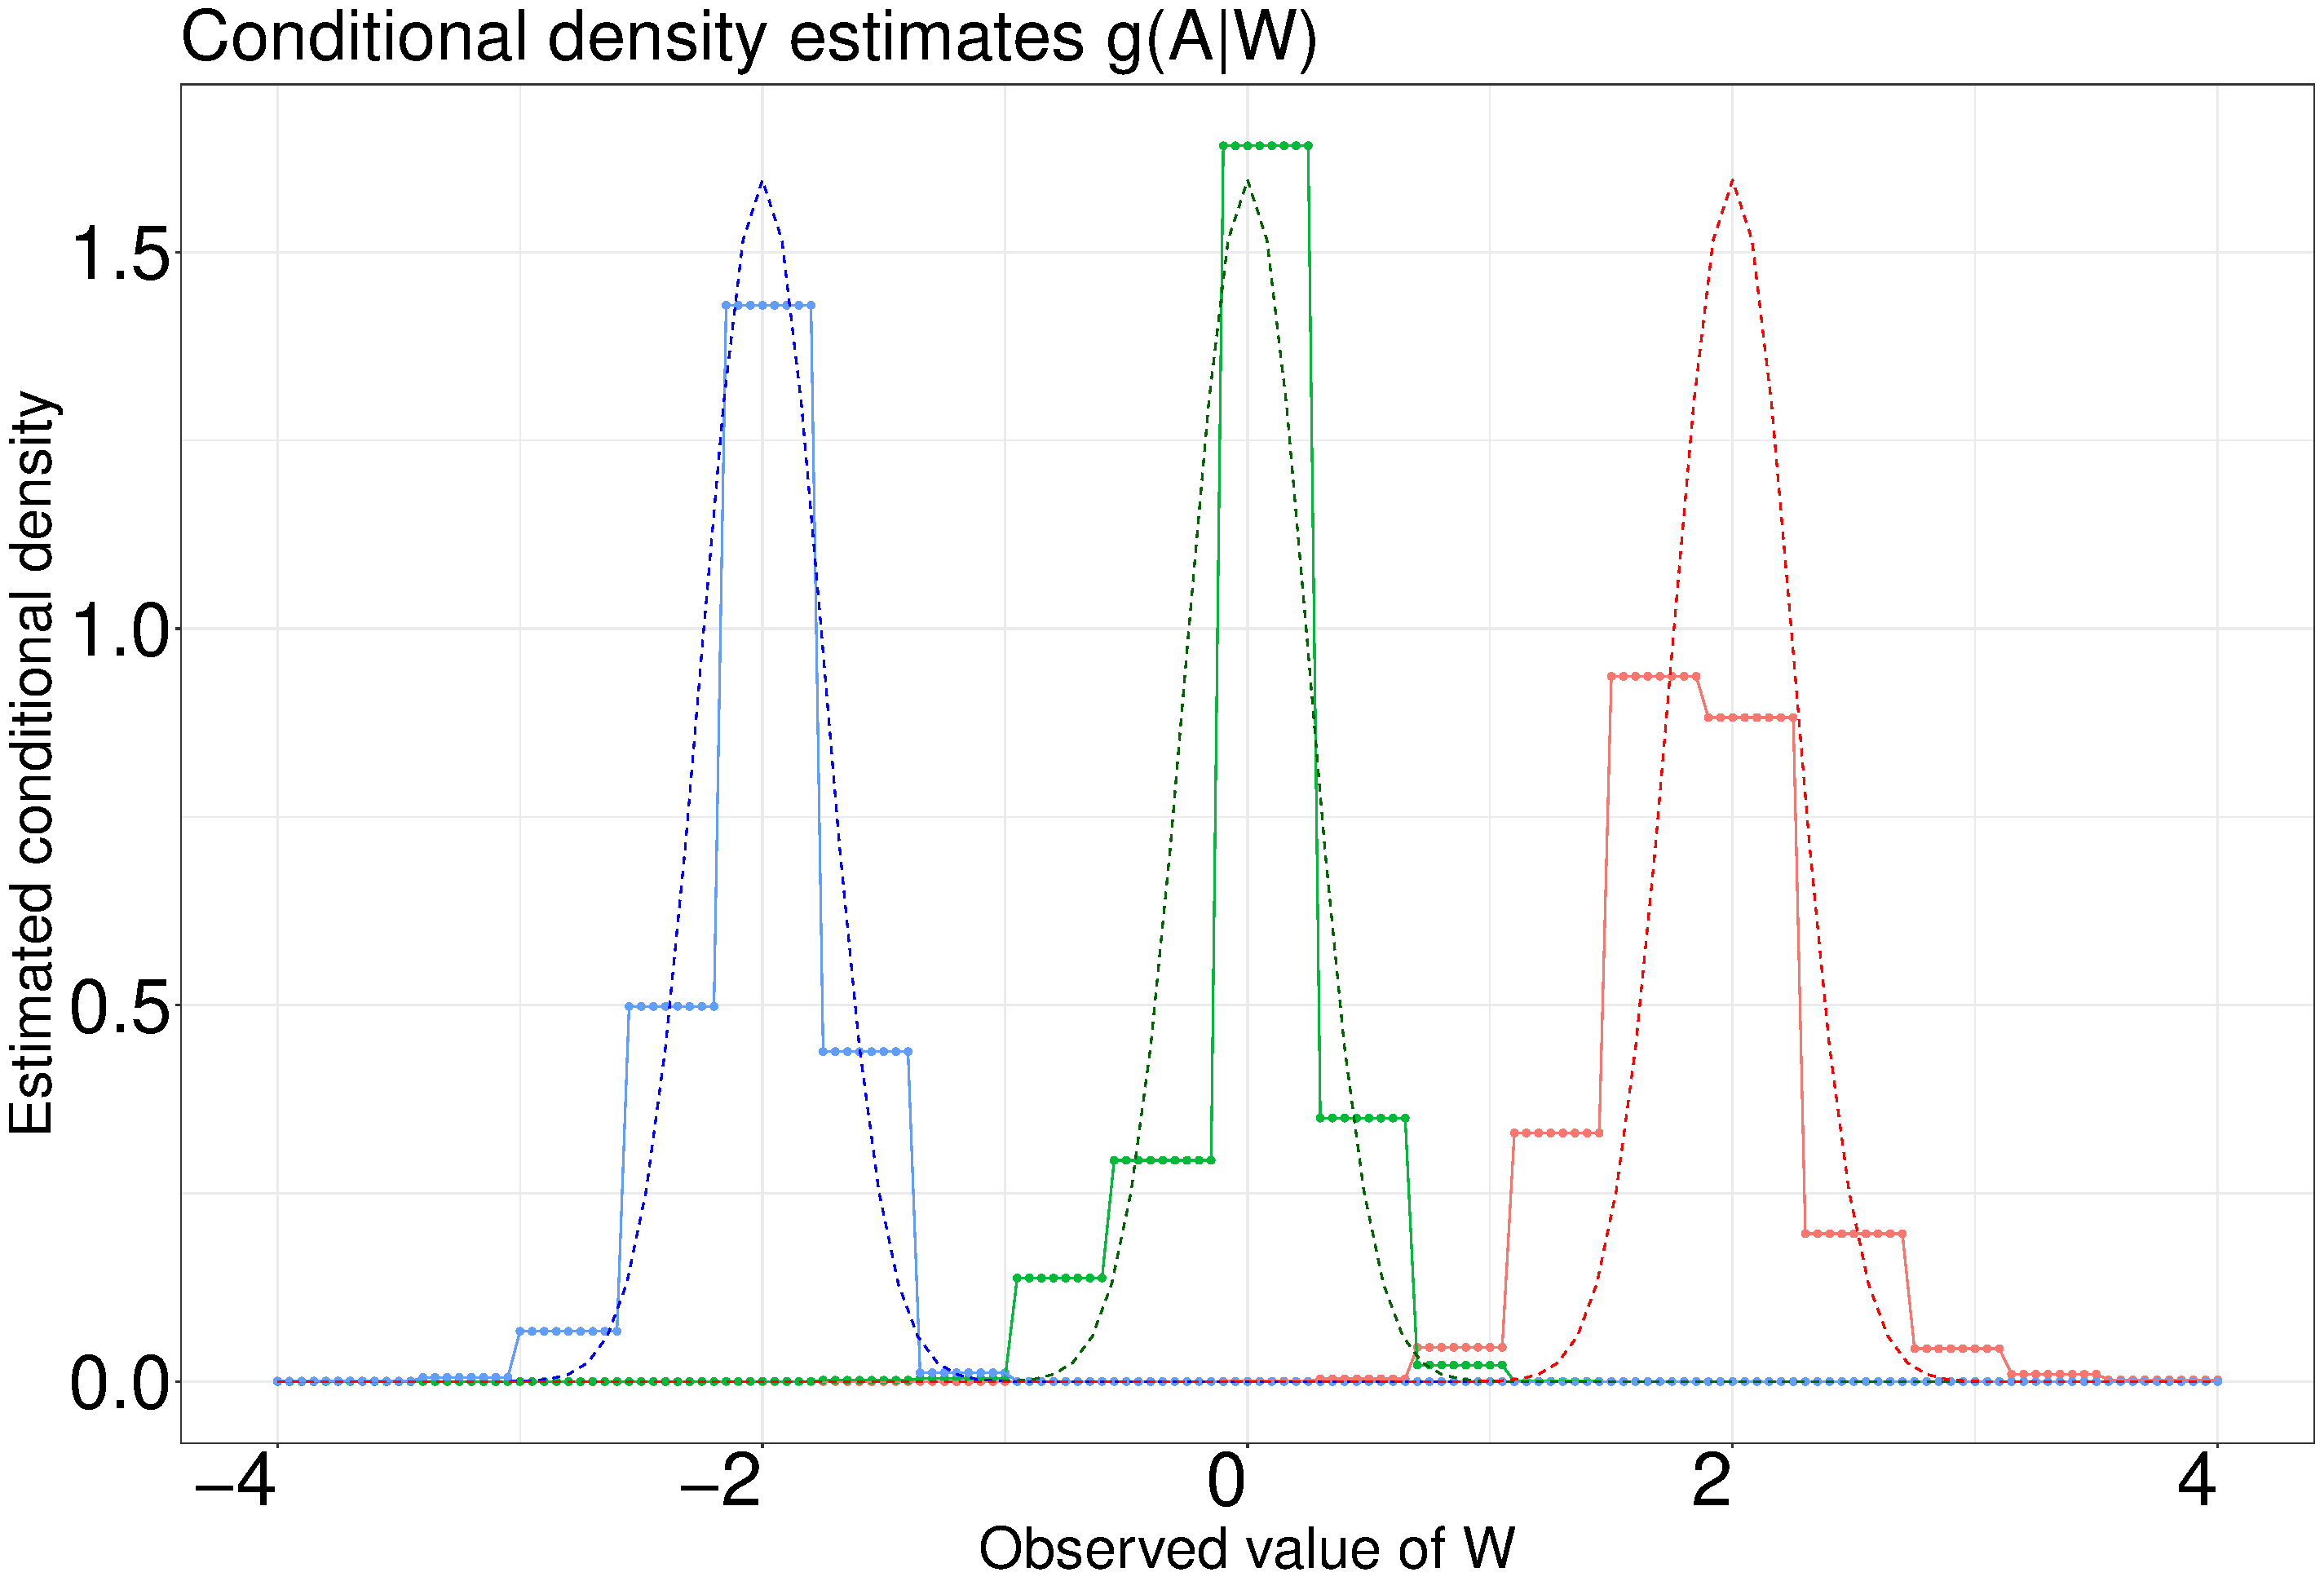
\includegraphics[scale=0.28]{haldensify_est}
  \caption{Conditional density estimates evaluated at different values of $W$,
    compared to the reference distribution at those same values.}
  \label{fig:haldensify_est}
\end{figure}
